This portion of the experiment is concerned with the cavity, which  is a quarter wavelength coaxial resonator.

We note that the cavity only resonates at a particular frequency, at all other frequencies we will have a reflection of the voltage signal.

\subsection{Cavity Reflection}
First we test this by ramping through the $V_{tune}$ voltages, which equates to ramping through the frequencies as shown in Part \ref{partA} more specifically in equation \ref{V2F}.

An examples of such a graph is shown in Figure \ref{fig:scope3_raw}. We note that a raw $V_{tune}$ ramp is noisy as the oscilloscope does not output the required accuracy, so we take a linear fit of the $V_{tune}$. From this point onward unless otherwise stated, we will always present the $V_{tune}$ as frequency which has undergone a linear voltage fit and gone through the conversion shown in equation \ref{V2F}. 

\begin{figure}[H]
\centering
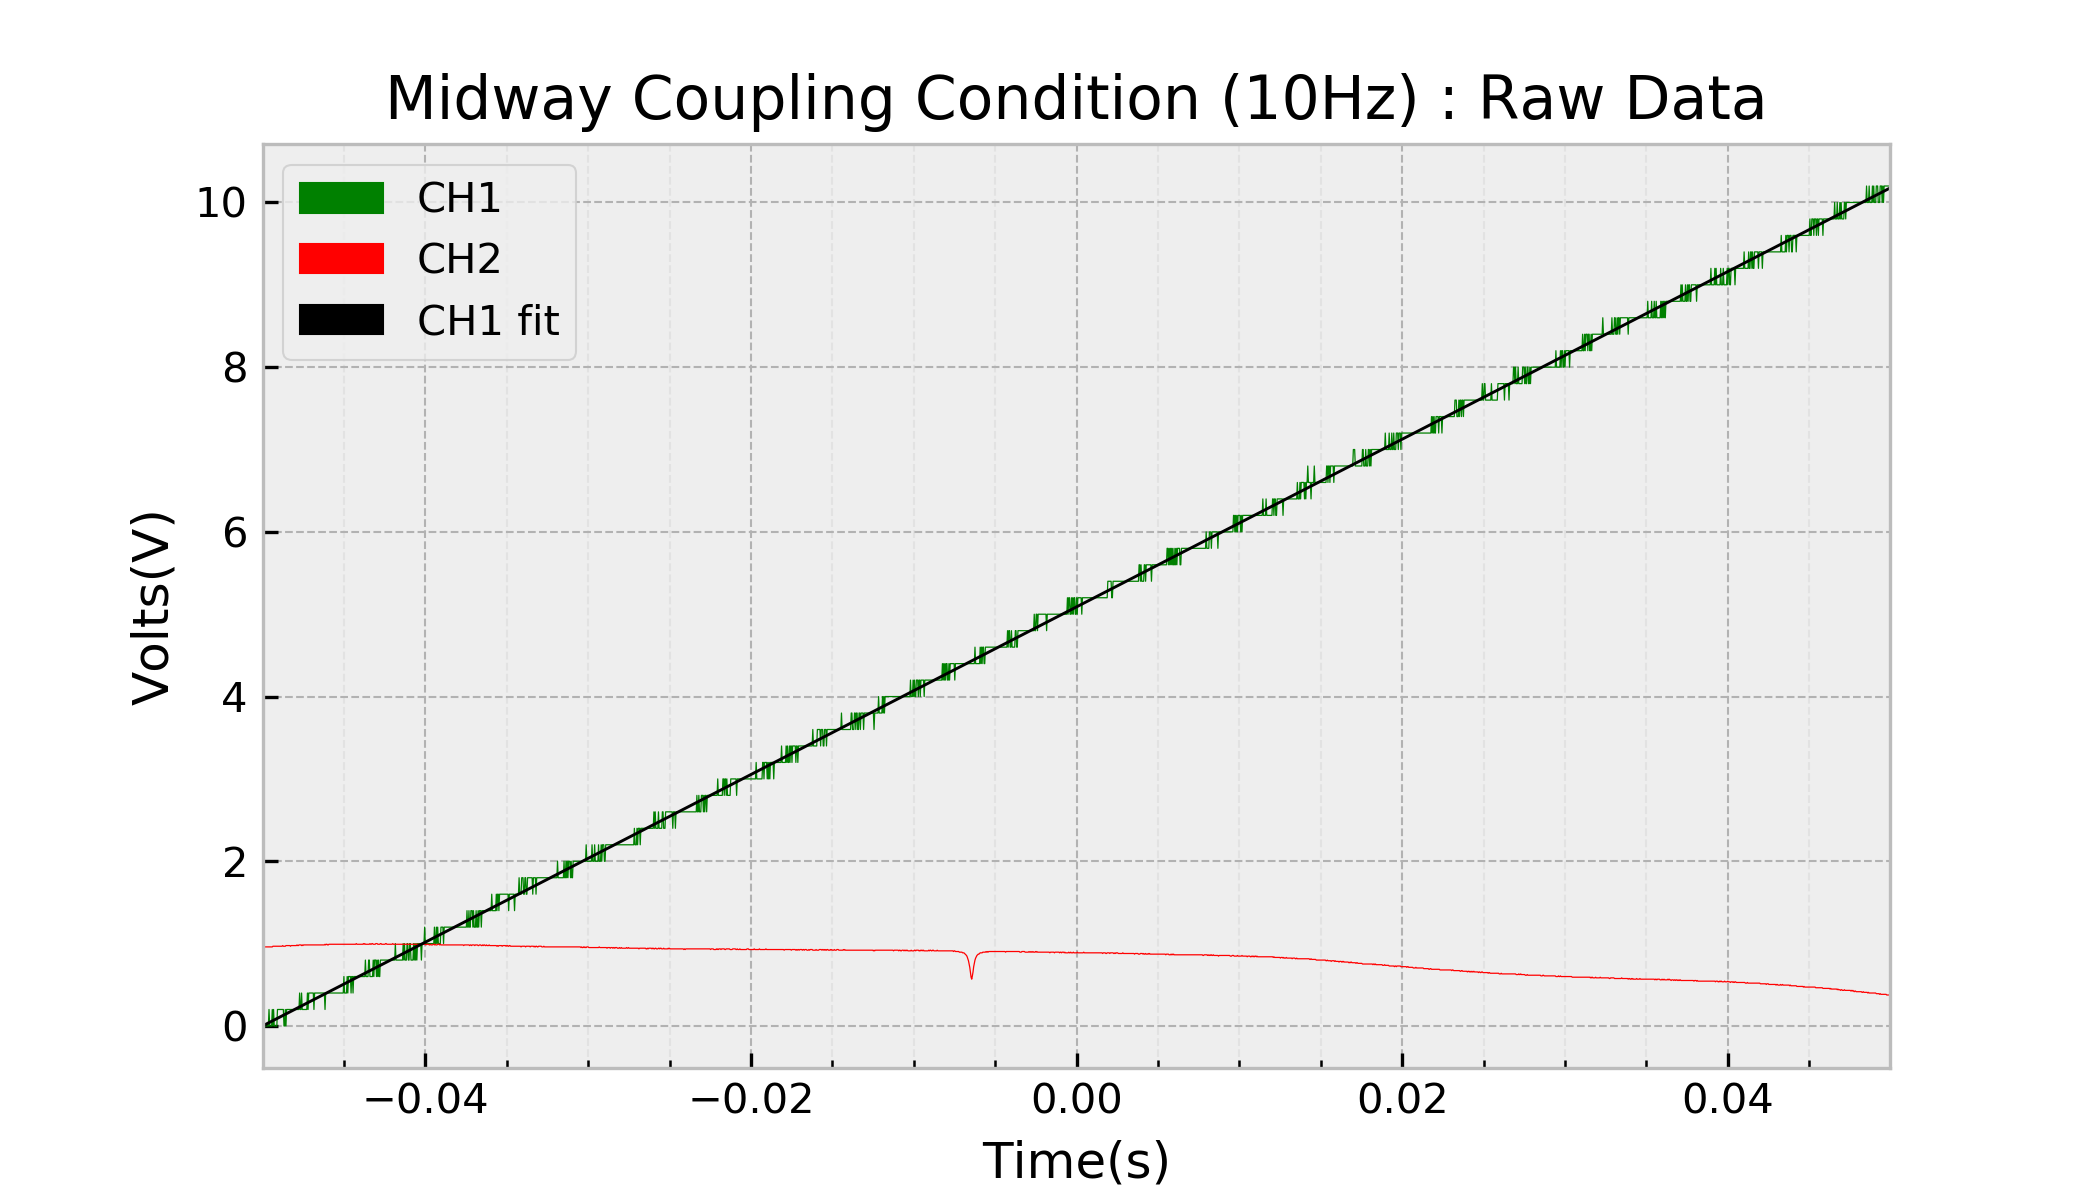
\includegraphics[width=0.75\textwidth]{figures/PartB/scope_3_raw.png}
\caption{Raw output of a cavity reflection, with an interpolated voltage scale shown}
\label{fig:scope3_raw}
\end{figure}

Once we have coupled the input loop into the cavity we can change the orientation to create different coupling conditions. Here we present a critical coupling condition in Figure \ref{fig:B_reflect_crit_10} and then we present a minimal coupling condition \ref{fig:B_reflect_min}. We note that these occur at 90$^\circ$ away from one another when turning the input coupling loop.

We can see the resonance frequency which is labelled in Figure \ref{fig:B_reflect_crit_10}, scanning at 10Hz however scanning at a slower rate of 2Hz and decreasing our time bounds to more closely view the resonance drop we can get a more accurate value for the resonance frequency. This is shown in Figure \ref{fig:B_reflect_crit_2}, and gives us a frequency value of 809.89 MHz with a voltage of 0.120 V. We note that the non-zero value of the peak implies that there are some imperfections which are involved with the reading, and the lower value found in Figure \ref{fig:B_reflect_crit_10} implies that the hand set value is not exactly a a critical coupling condition. However this will not alter the location of the peak, so it should not cause any further issues.

\begin{figure}[h!]
\centering
\begin{subfigure}[t]{.475\textwidth}
  \centering
  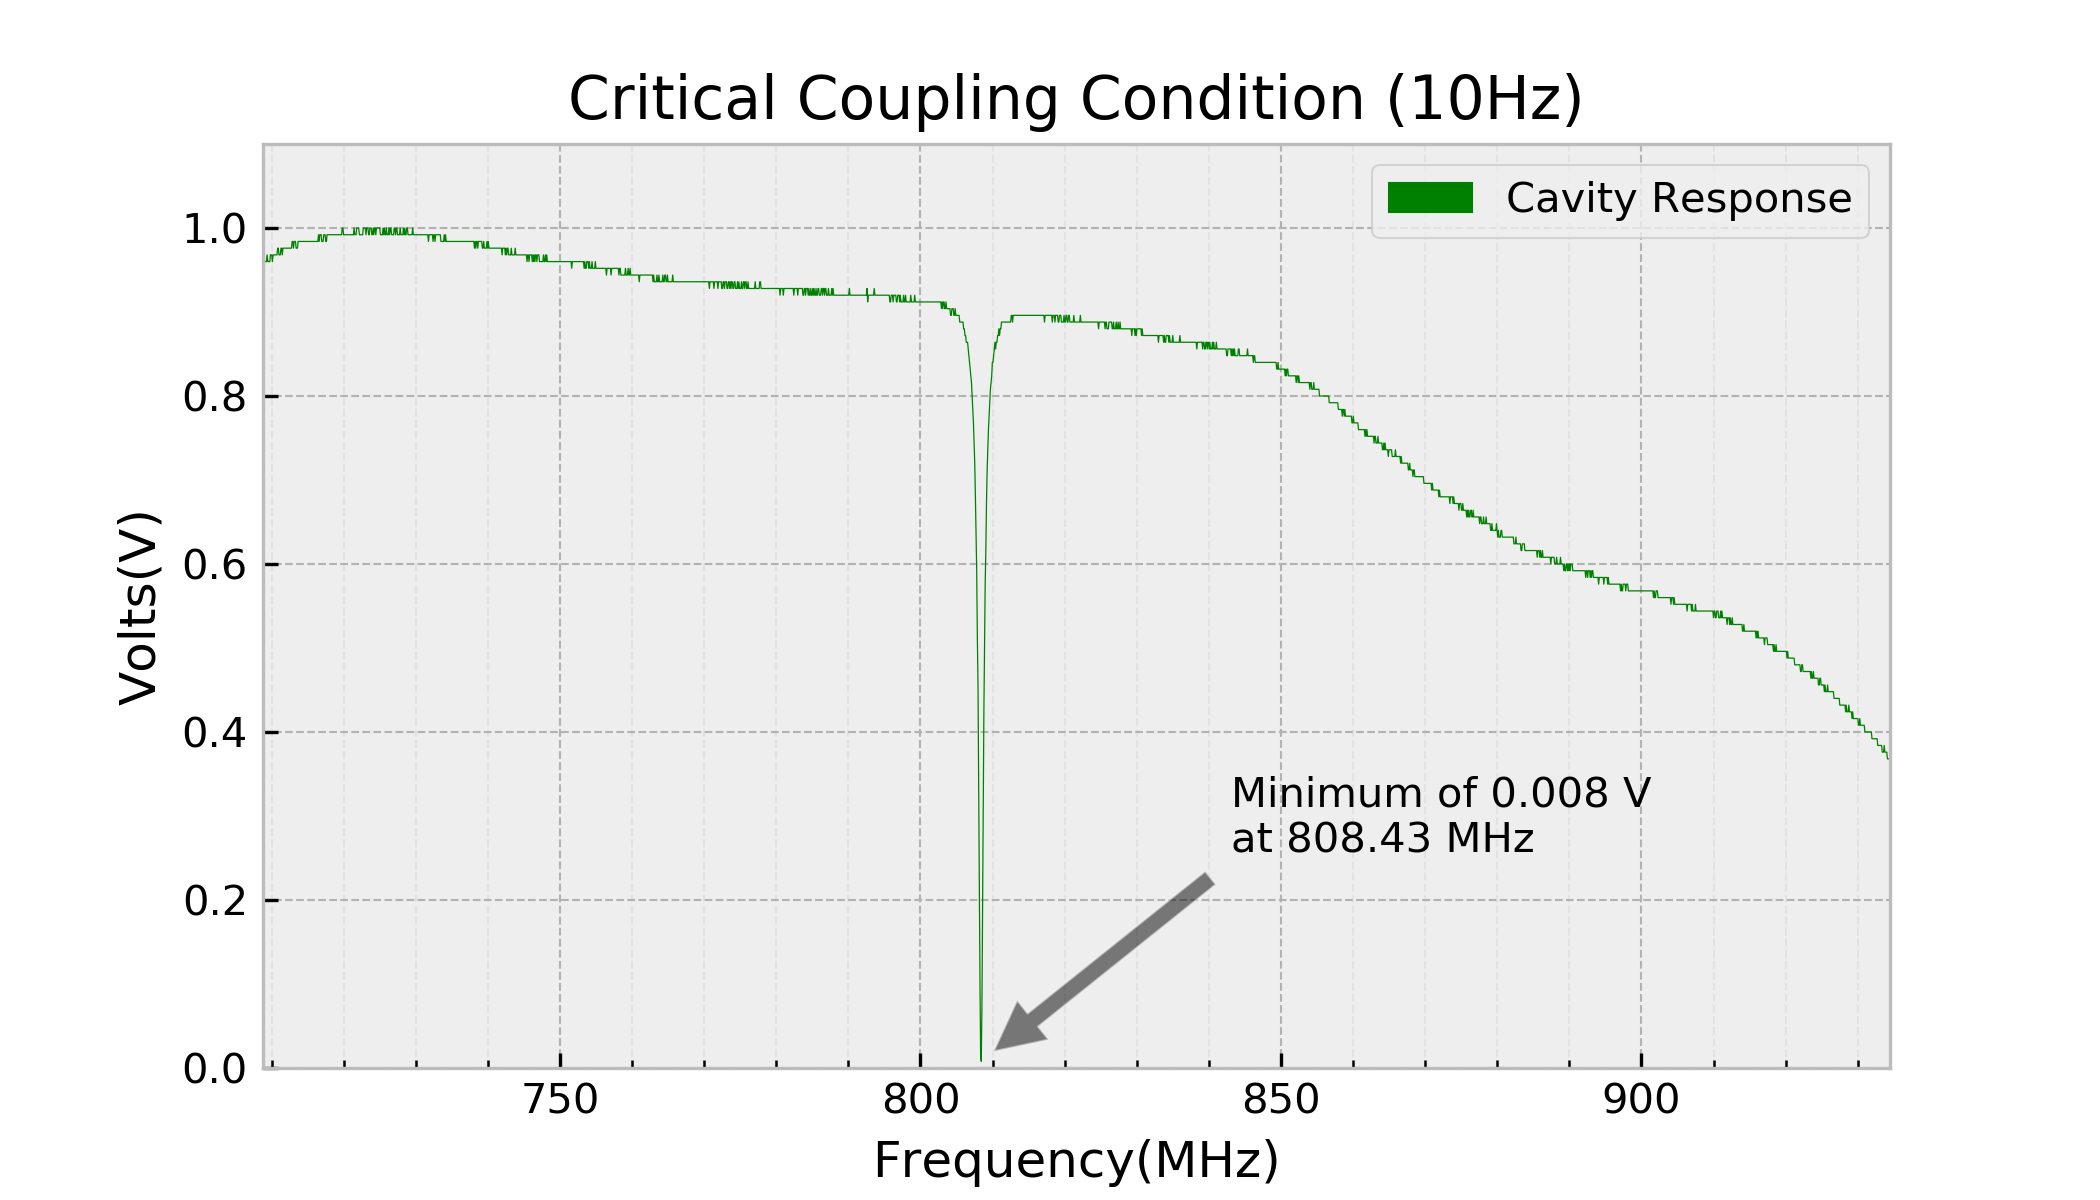
\includegraphics[width=0.95\textwidth]{figures/PartB/scope_1.png}
  \caption{Critical coupling condition for reflection of the cavity at a voltage ramp of 10Hz}
 \label{fig:B_reflect_crit_10}
\end{subfigure}\hfill
\begin{subfigure}[t]{.475\textwidth}
  \centering
  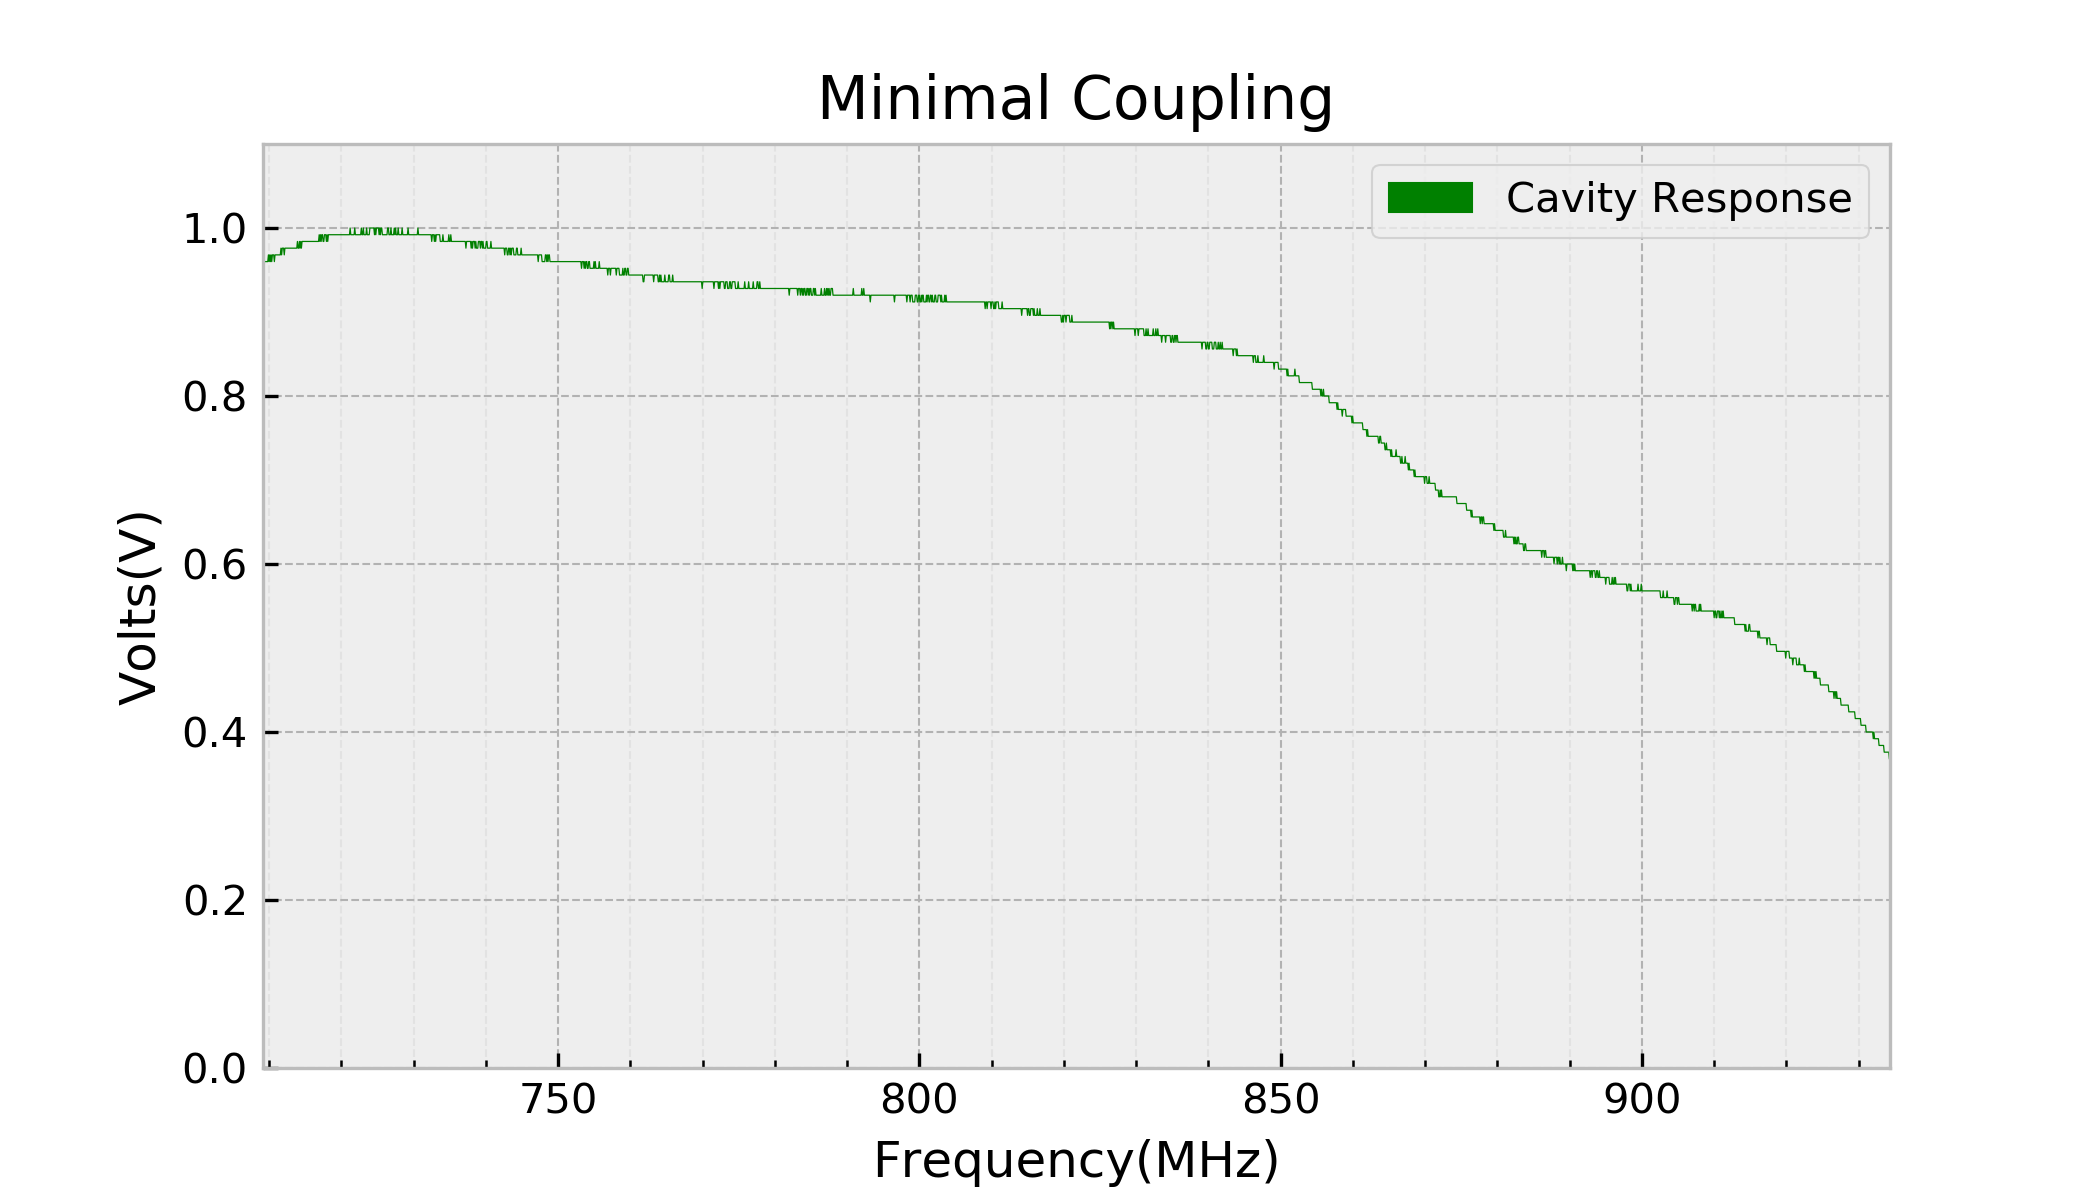
\includegraphics[width=0.95\textwidth]{figures/PartB/scope_2.png}
  \caption{Minimal coupling condition for reflection of the cavity at a voltage ramp of 10Hz}
\label{fig:B_reflect_min}
\end{subfigure}
\caption{Different coupling conditions leading to different reflections.}
\label{fig:B_reflect_conditions}
\end{figure}

\begin{figure}[H]
\centering
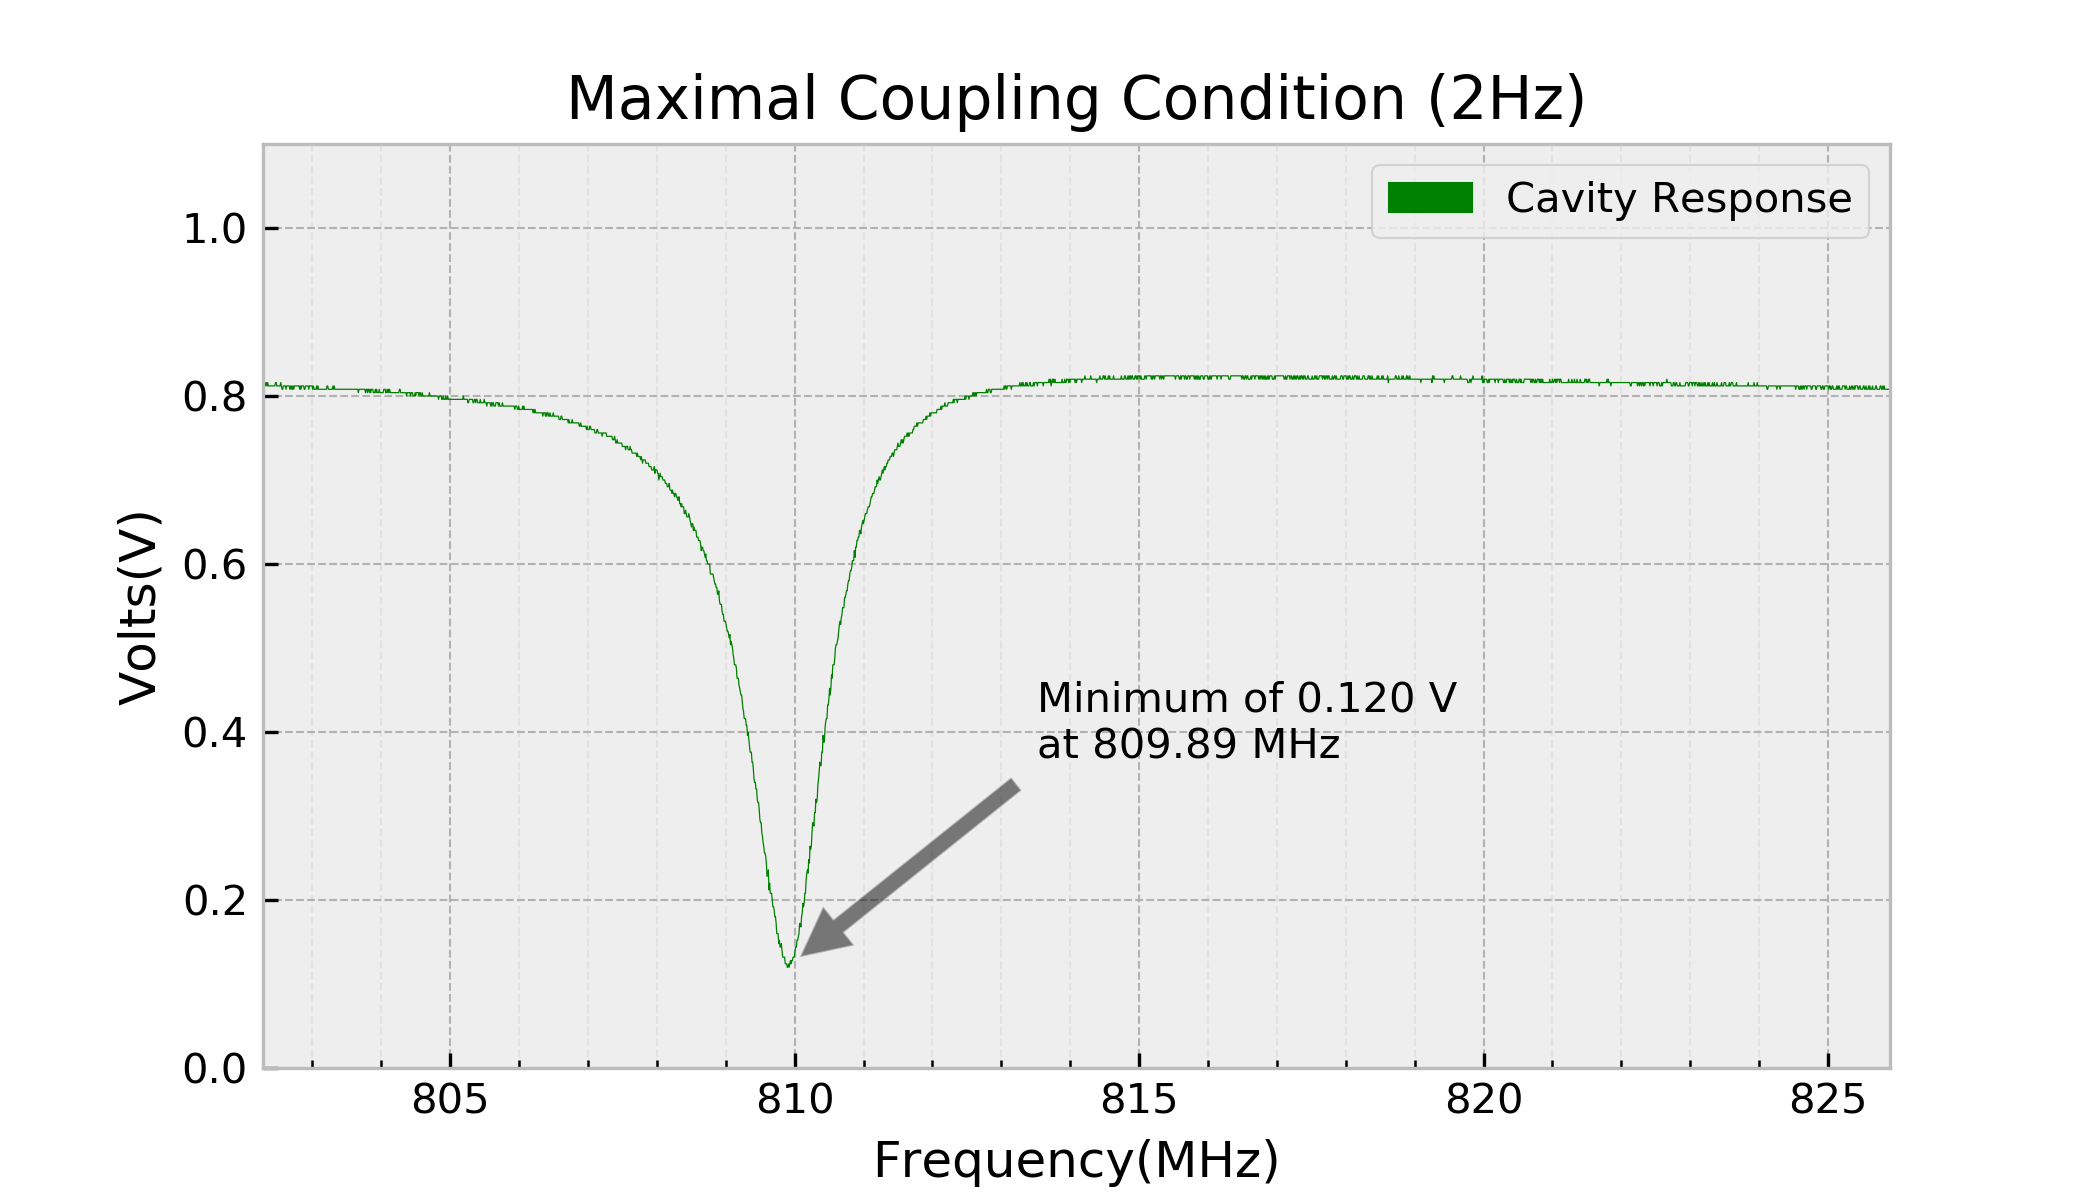
\includegraphics[width=0.75\textwidth]{figures/PartB/scope_4.png}
\caption{Critical coupling condition for reflection of the cavity at a voltage ramp of 2Hz}
\label{fig:B_reflect_crit_2}
\end{figure}
\clearpage

\subsection{Cavity Transmission}

We can then change the setup to allow for transmission. This is done according to the lab manual \cite{LabProcedure}. Therefore we then change the output loop to scan over the transmission conditions. This is shown in Figure \ref{fig:B_trans_raw} We can see that the received transmitted data is altered by the changes in the coupling loop's orientation, but nothing else is significantly altered.

\begin{figure}[h!]
\centering
\begin{subfigure}[t]{.475\textwidth}
  \centering
  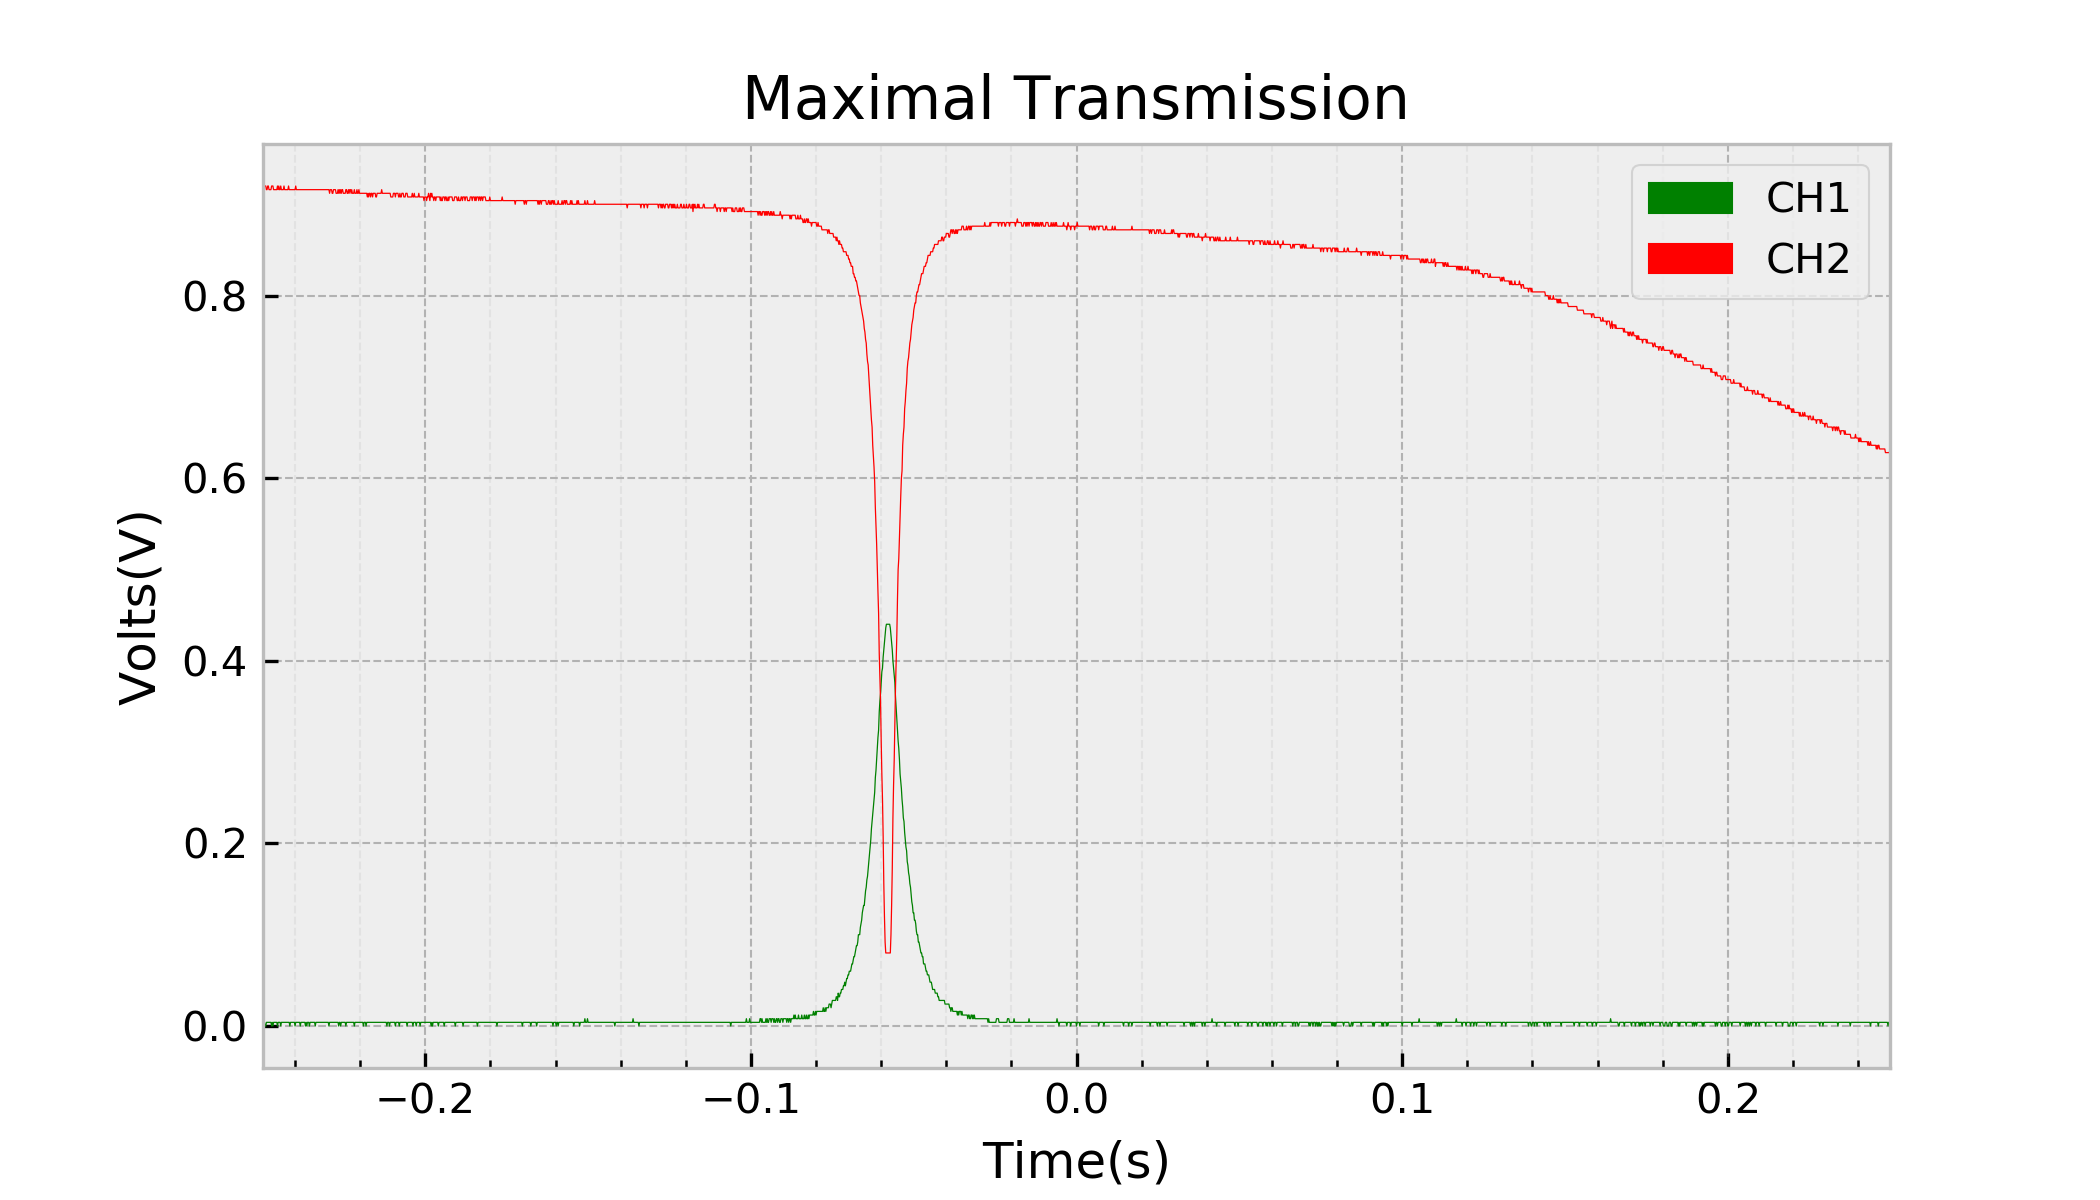
\includegraphics[width=0.95\textwidth]{figures/PartB/scope_6.png}
  \caption{Raw data of maximal transmission scan.}
 \label{fig:B_trans_max_raw}
\end{subfigure}\hfill
\begin{subfigure}[t]{.475\textwidth}
  \centering
  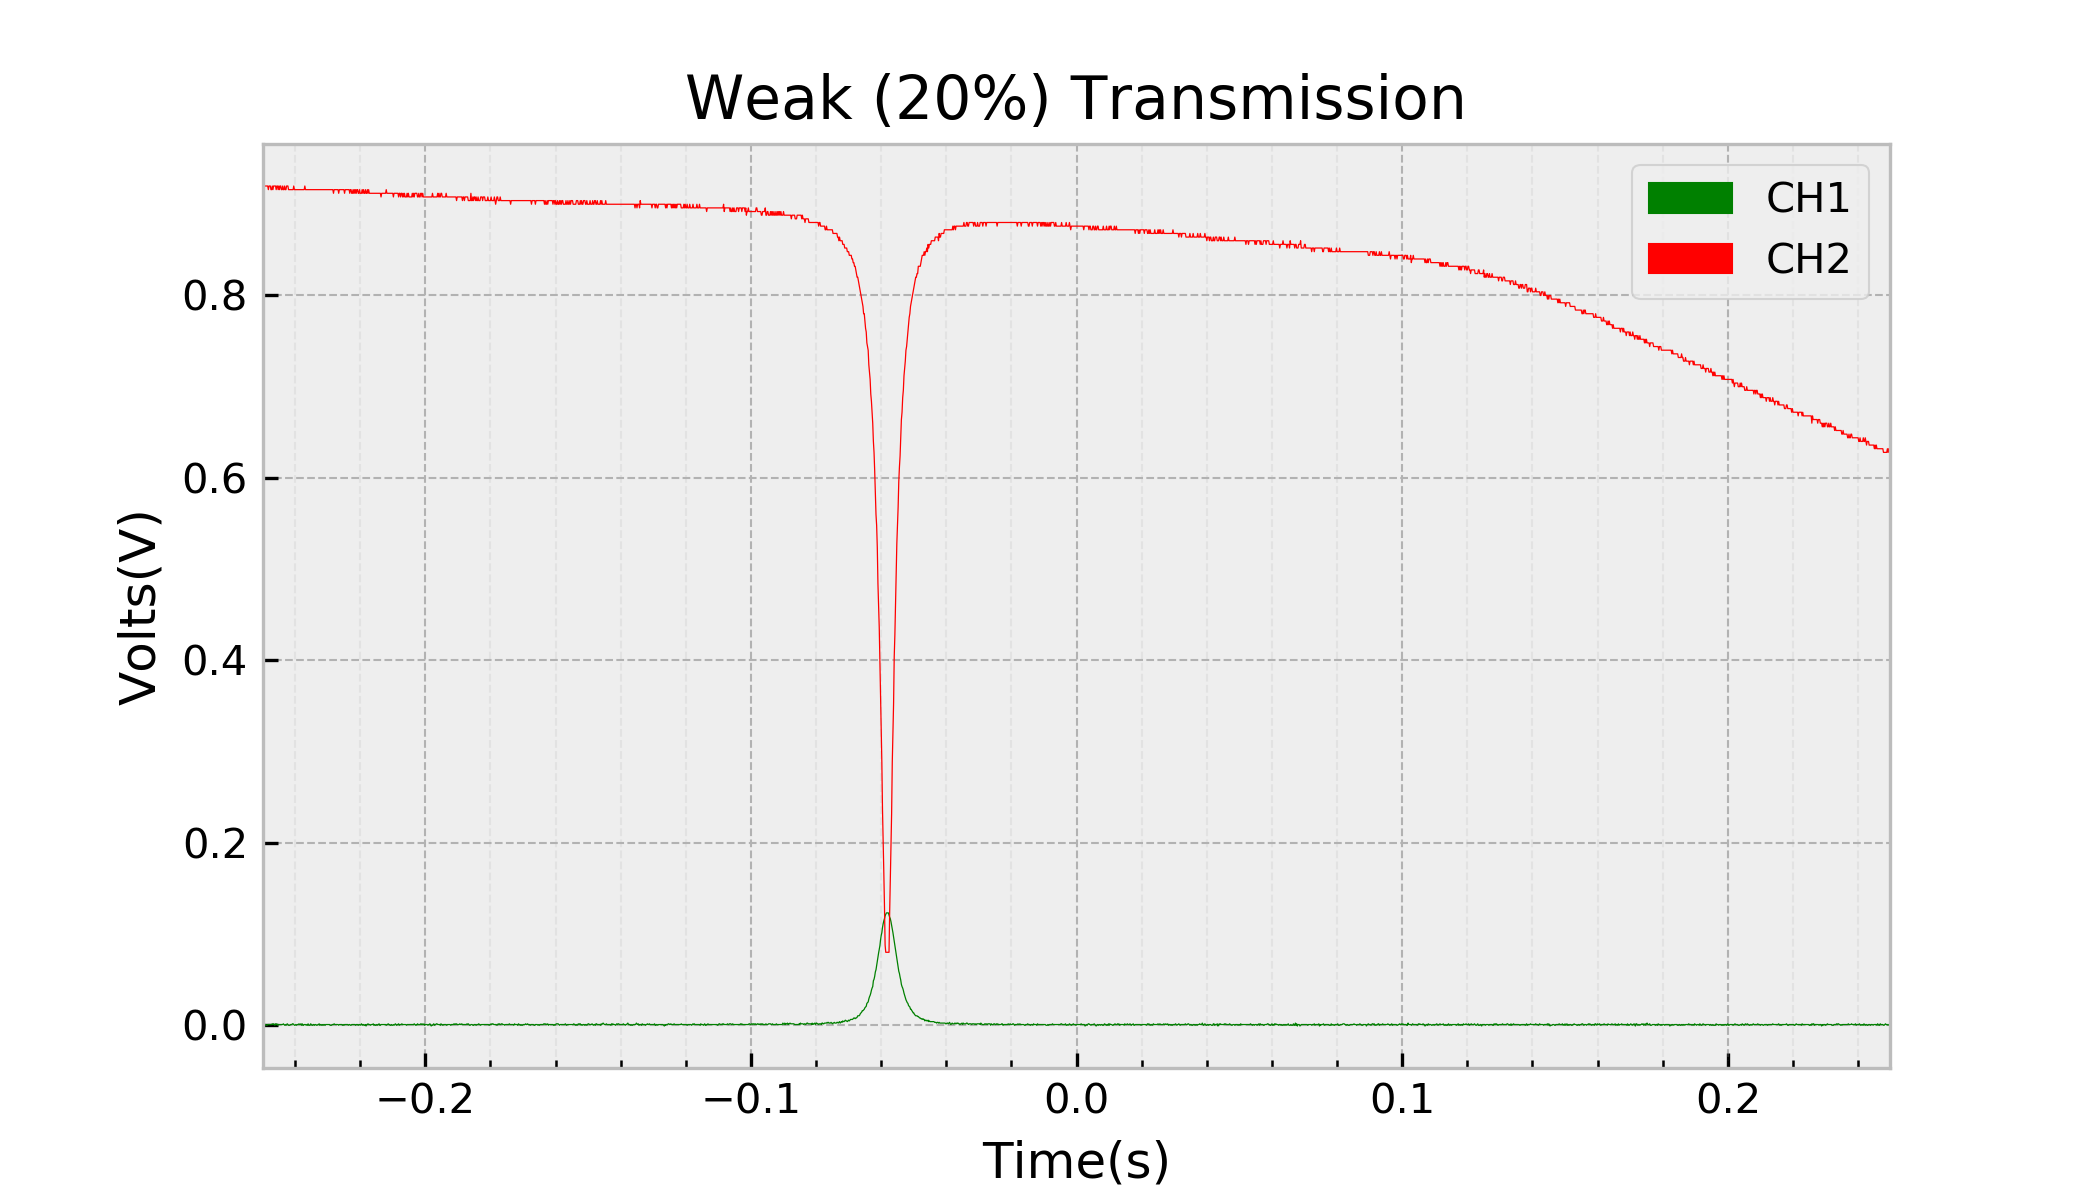
\includegraphics[width=0.95\textwidth]{figures/PartB/scope_5.png}
  \caption{Raw data of weak coupling transmission scan.}
\label{fig:B_trans_weak_raw}
\end{subfigure}
\caption{Transmission scopes, showing cavity transmission at different coupling conditions}
\label{fig:B_trans_raw}
\end{figure}

We then take a value which is 20\% of the maximal transmitted signal to create a weak coupling condition. This is completed as the impedance of the oscilloscope can affect resonance. This weak coupling condition is roughly found to occur at 15$^\circ$ away from minimal transmission settings. We will set the coupling loops in this configuration for the remainder of the lab.

\begin{figure}[h!]
\centering
\begin{subfigure}[t]{.475\textwidth}
  \centering
  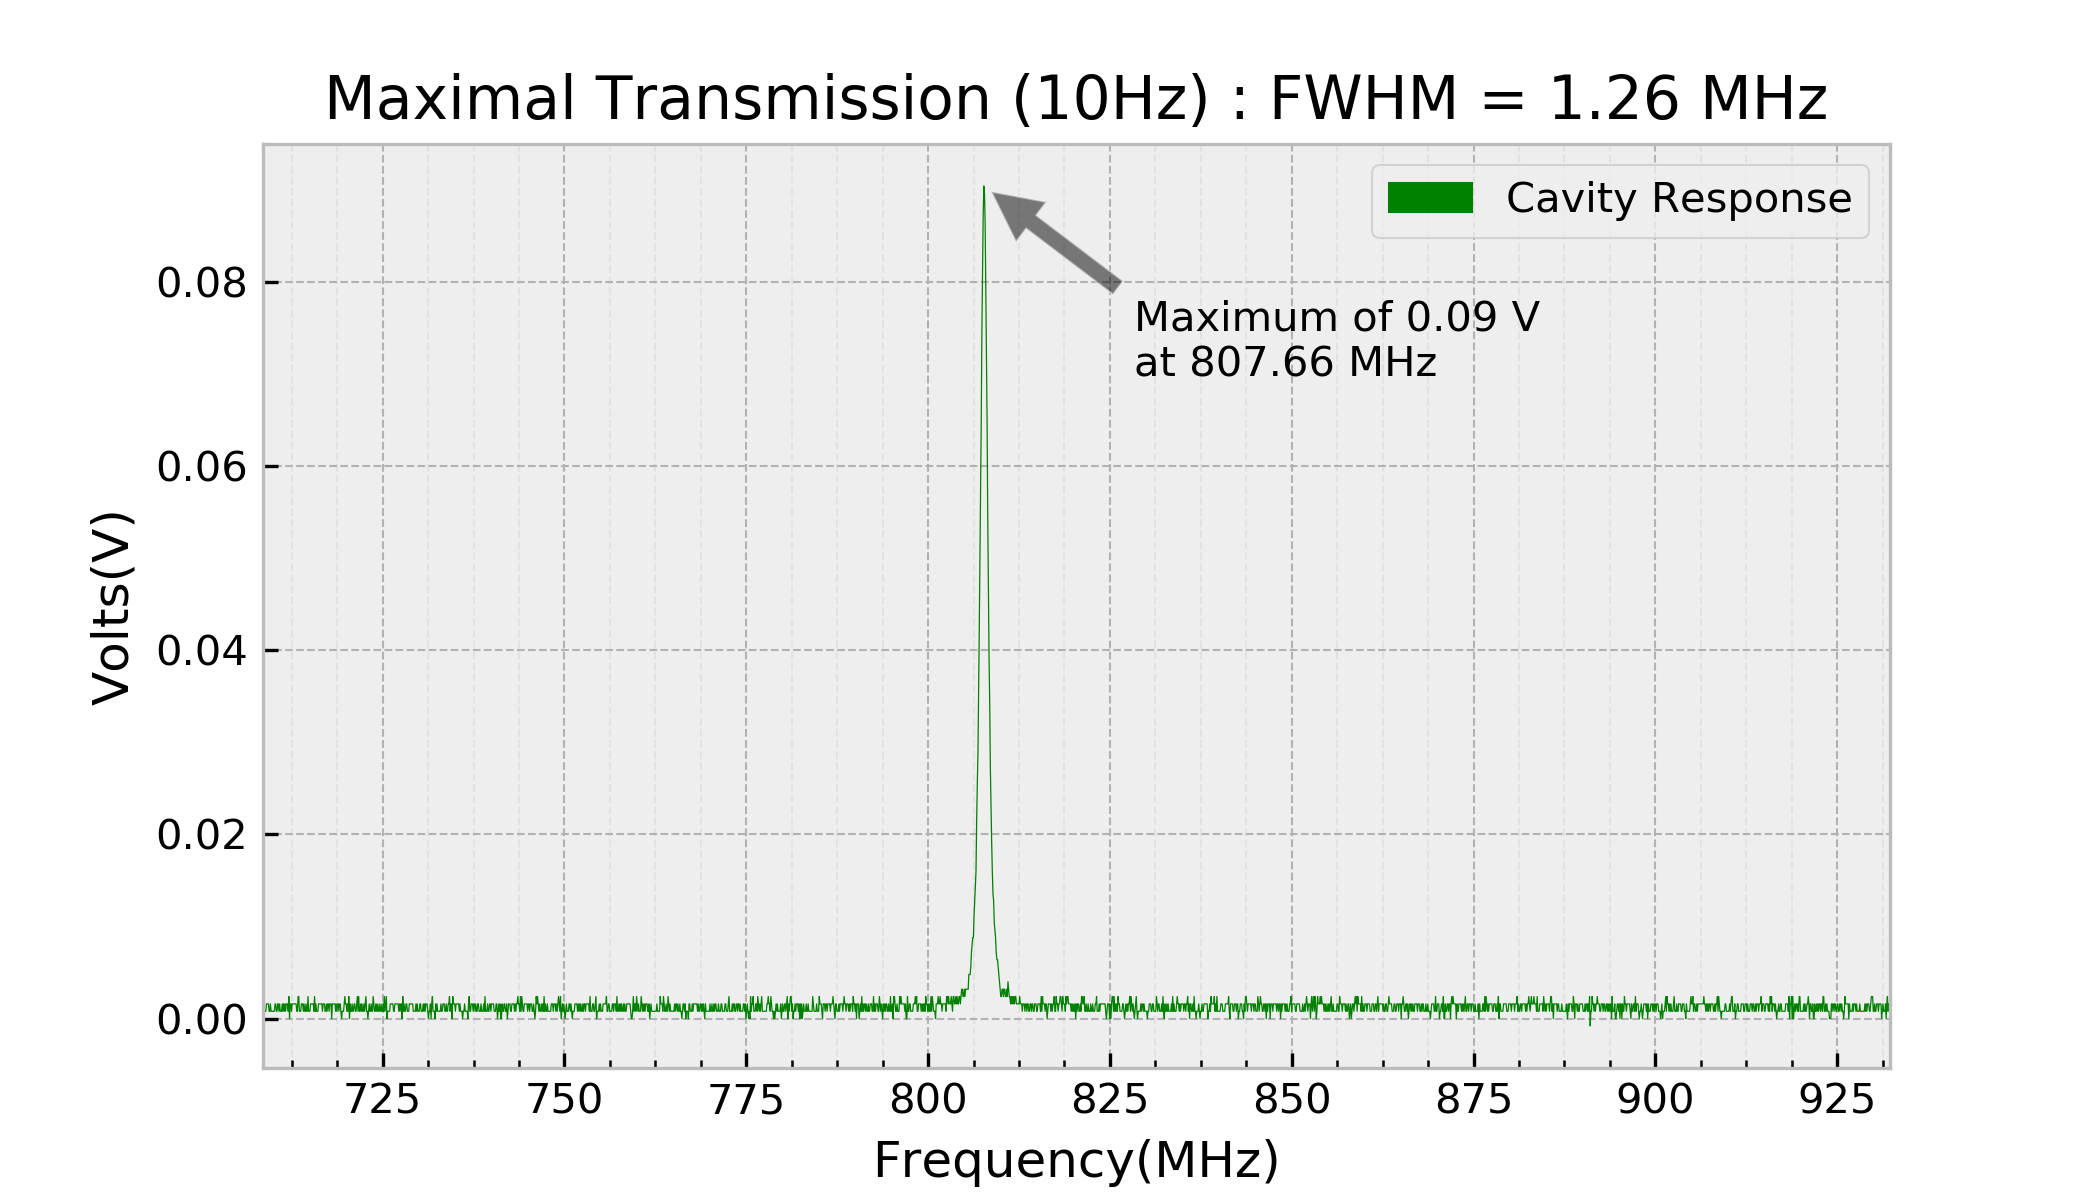
\includegraphics[width=0.95\textwidth]{figures/PartB/scope_10.png}
  \caption{Transmission signal at 10Hz input}
 \label{fig:B_trans_10}
\end{subfigure}\hfill
\begin{subfigure}[t]{.475\textwidth}
  \centering
  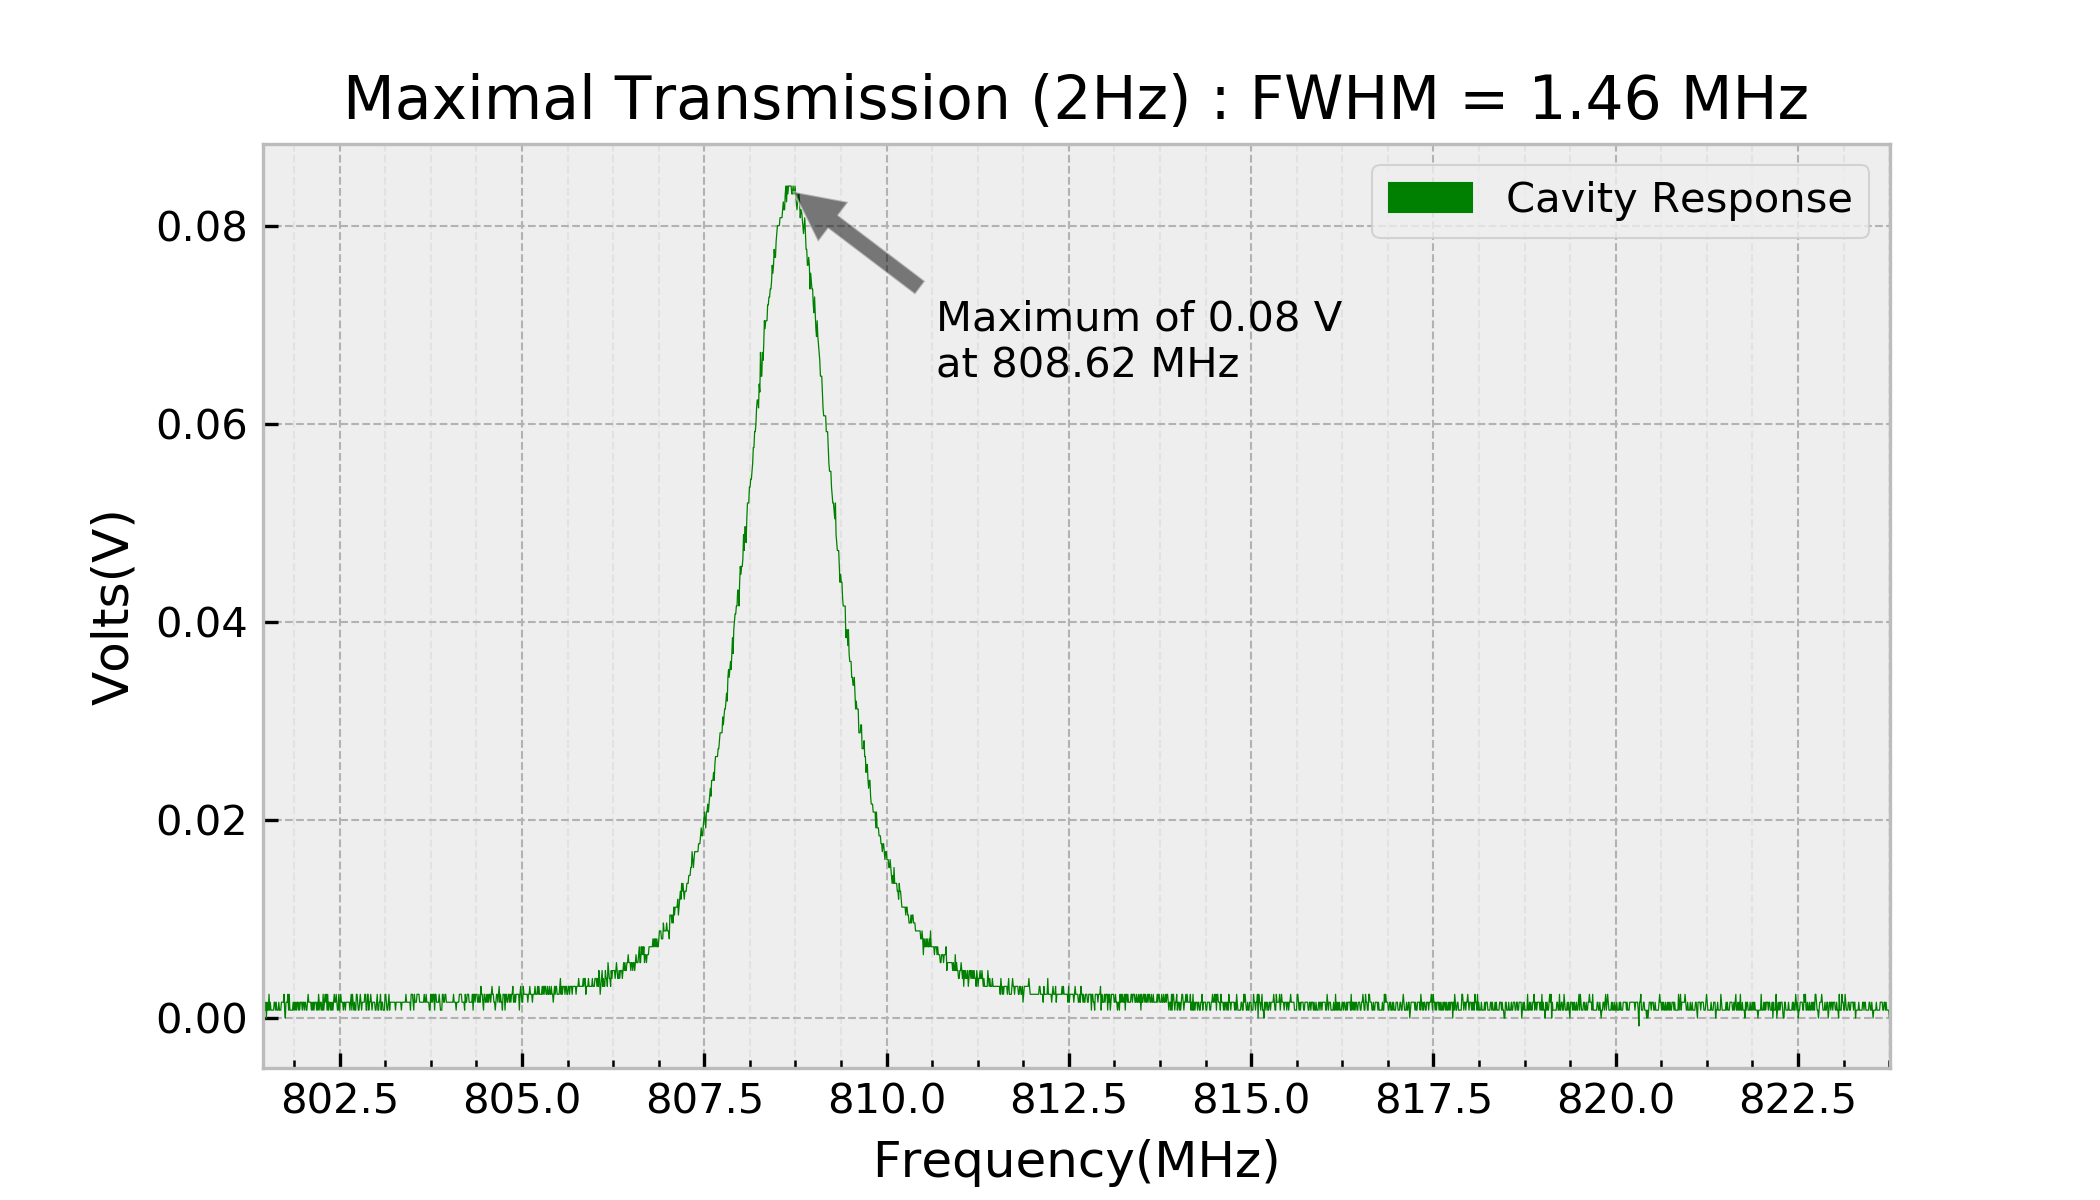
\includegraphics[width=0.95\textwidth]{figures/PartB/scope_8.png}
  \caption{Transmission signal at 2Hz input}
\label{fig:B_trans_2}
\end{subfigure}
\caption{Transmission signals at different repeat frequencies}
\label{fig:B_trans}
\end{figure}

We determine that the resonant frequency of the cavity is at 808.62 MHz from our more accurate graph at 2Hz, but we then see that the less accurate graph gives us a different value of resonance at 807.66 MHz, it is expected that we will have some difference as the cavity must take some period of time to achieve equilibrium, but the 10Hz value is suggested in the lab manual does not appear to be appropriate. We will state that the resonant frequency is 808 $\pm$ 2 MHz due to this difference in found resonant frequencies. We also find that the Full Width at Half Maximum (FWHM) of the signal is 1.5 $\pm$ .2 MHz, which was found through a custom script \cite{code}.

From this we are able to calculate a Quality factor of 560 $\pm$ 40 which is calculated based off of the formula of $Q_\ell = \frac{\text{Resonant Frequency}}{FWHM}$. We note that the error in this calculation is quite large as the FWHM from our two scans do not agree, hence we state a large error. From this measure we are able to calculate a graph of $|\Gamma|^2$ vs frequency, which we show in Figure \ref{fig:gamma}. This is calculated through the formula, where $\omega_o$ is the angular resonance frequency and $\Delta\omega$ is the angular distance from resonance.

\begin{equation}
    |\Gamma|^2 = 1\; -\; \frac{1}{1-4 Q_\ell^2 (\Delta\omega/\omega_o)^2}
\end{equation}

From this $|\Gamma|^2$ we are able to calculate an expected or theoretical graph of the reflected power, first we note that the power relationship must be computed which is based off of the experimentally found voltage to power relation given to us in the lab manual \cite{LabProcedure}. After translating voltage we use the $P_{input}$ as the inputted signal without reflection, which can be seen in the minimal coupling condition (Figure \ref{fig:B_reflect_min}). We show this calculated reflection power in Figure \ref{fig:raw_reflect_calc}, we note that the found resonance frequency of this graph is used in calculations rather than the 2Hz signal to better compare the graphs. 

\begin{figure}[h!]
\centering
\begin{subfigure}[t]{.475\textwidth}
  \centering
  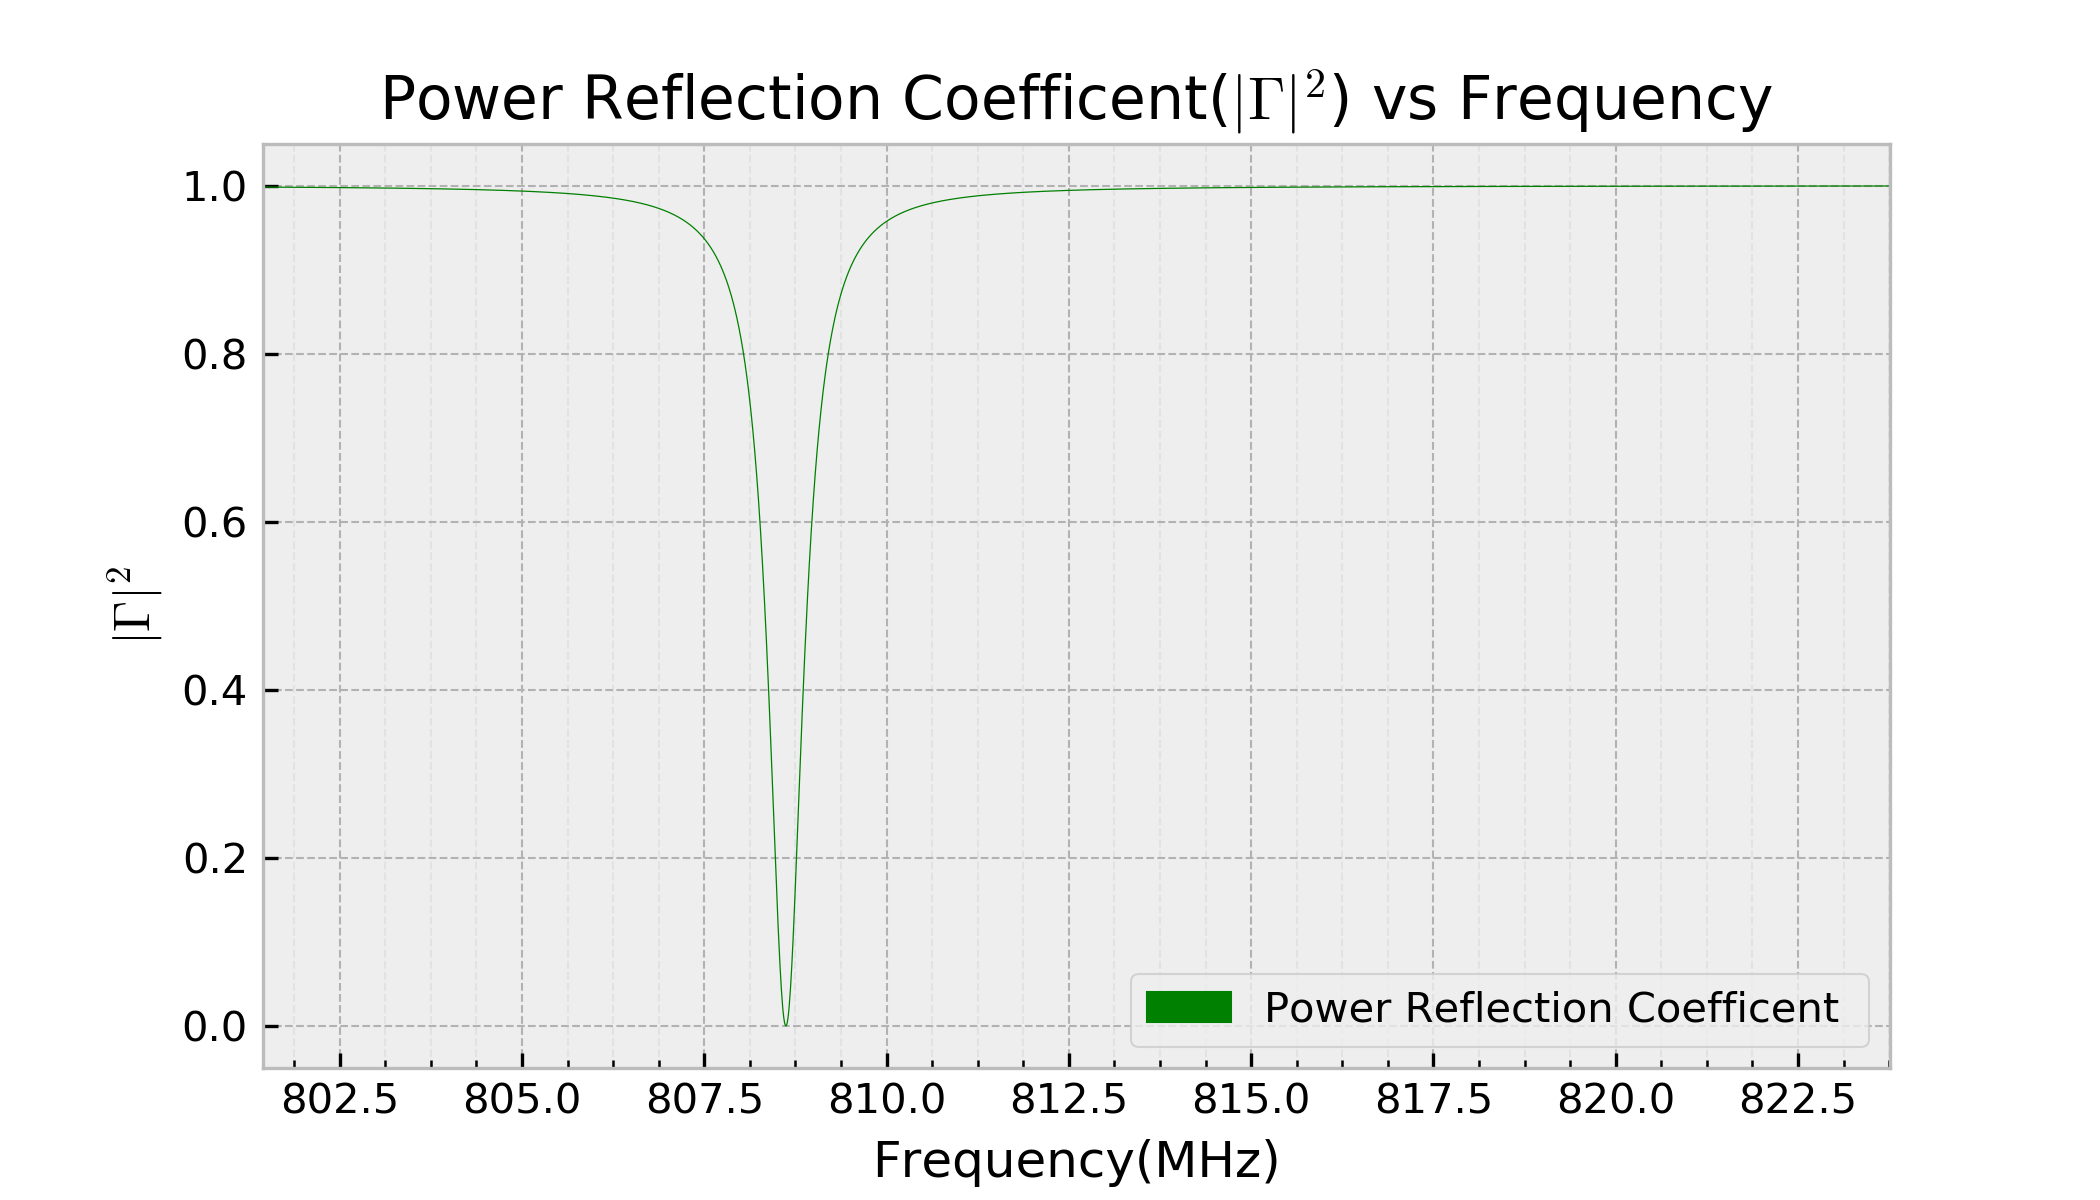
\includegraphics[width=0.95\textwidth]{figures/PartB/gamma.png}
  \caption{Calculated $|\Gamma|^2$ values vs frequency}
 \label{fig:gamma}
\end{subfigure}\hfill
\begin{subfigure}[t]{.475\textwidth}
  \centering
  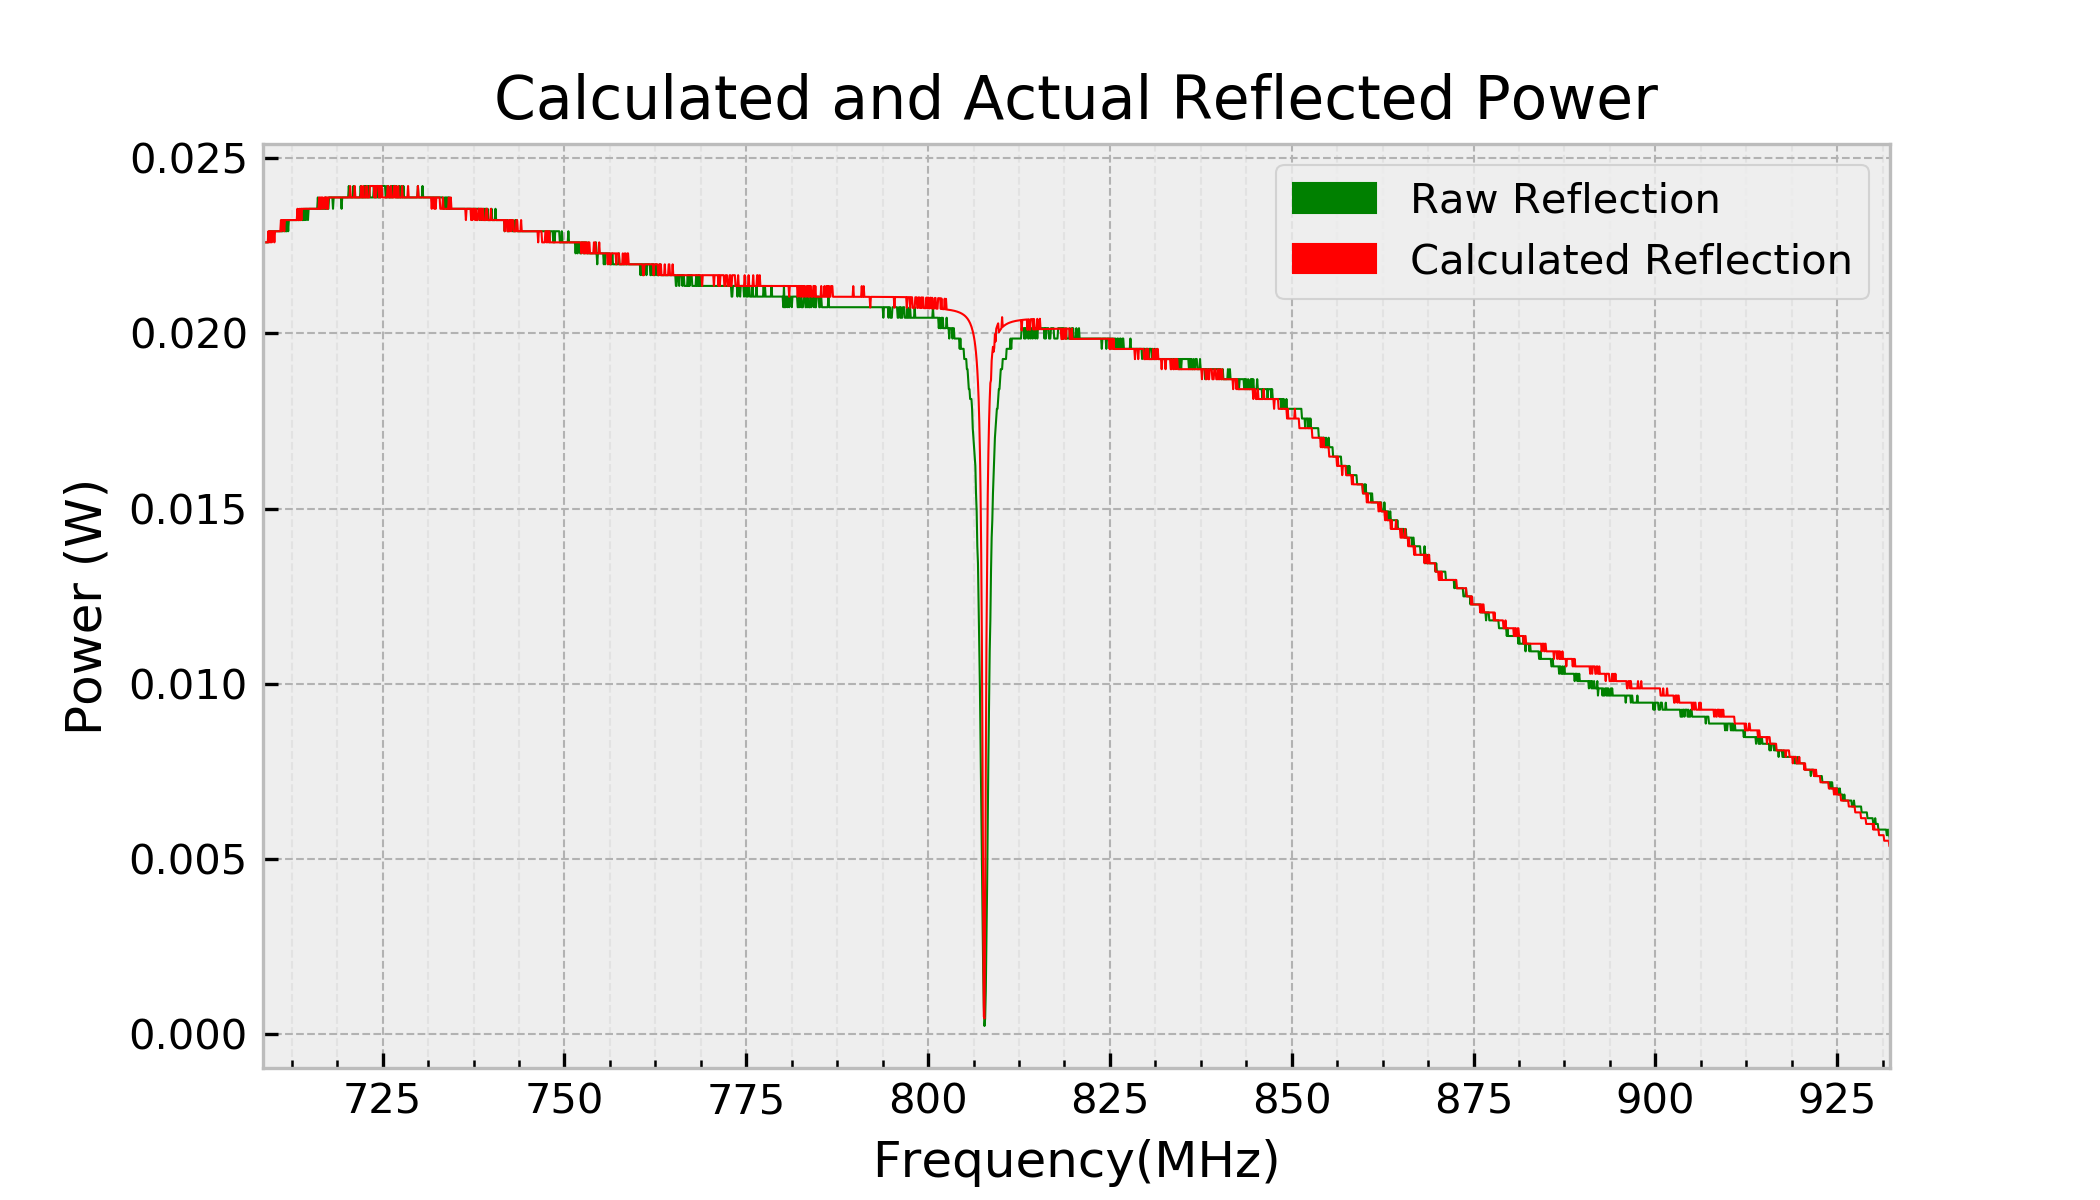
\includegraphics[width=0.95\textwidth]{figures/PartB/reflect_raw.png}
  \caption{Calculated vs Actual resonance conditions to compare the quality of the fit, original data also shown in Figure \ref{fig:B_reflect_crit_10}}
\label{fig:raw_reflect_calc}
\end{subfigure}
\caption{Gamma calculation and comparison graphs}
\label{fig:gamma}
\end{figure}

We also note that in Figure \ref{fig:raw_reflect_calc} we see a large amount of noise, to reduce this and see the underlying signal we use a Savitzky-Golay filter. The results of this are shown in Figure \ref{fig:raw_reflect_filt}. We see that generally the shape of the signal is preserved, with a couple of deviations, but the largest effect is seen at resonance. This deviation at resonance shows that the resonance peak is broader than the calculated resonance. This effect is emphasized in Figure \ref{fig:reflect_sub} where we subtract the calculated signal from the raw signal and filter it to show the difference in signal. We see from this that it is 10MHz broader than expected and the difference accounts for approximately 30\% of the signal at peak. The broadness of the signal is guessed to be a lack of uniformity of the signal. Non-idealities of the cavity will shift the resonance slightly, which will cause a smearing of the inputted frequencies.

\begin{figure}[h!]
\centering
\begin{subfigure}[t]{.475\textwidth}
  \centering
  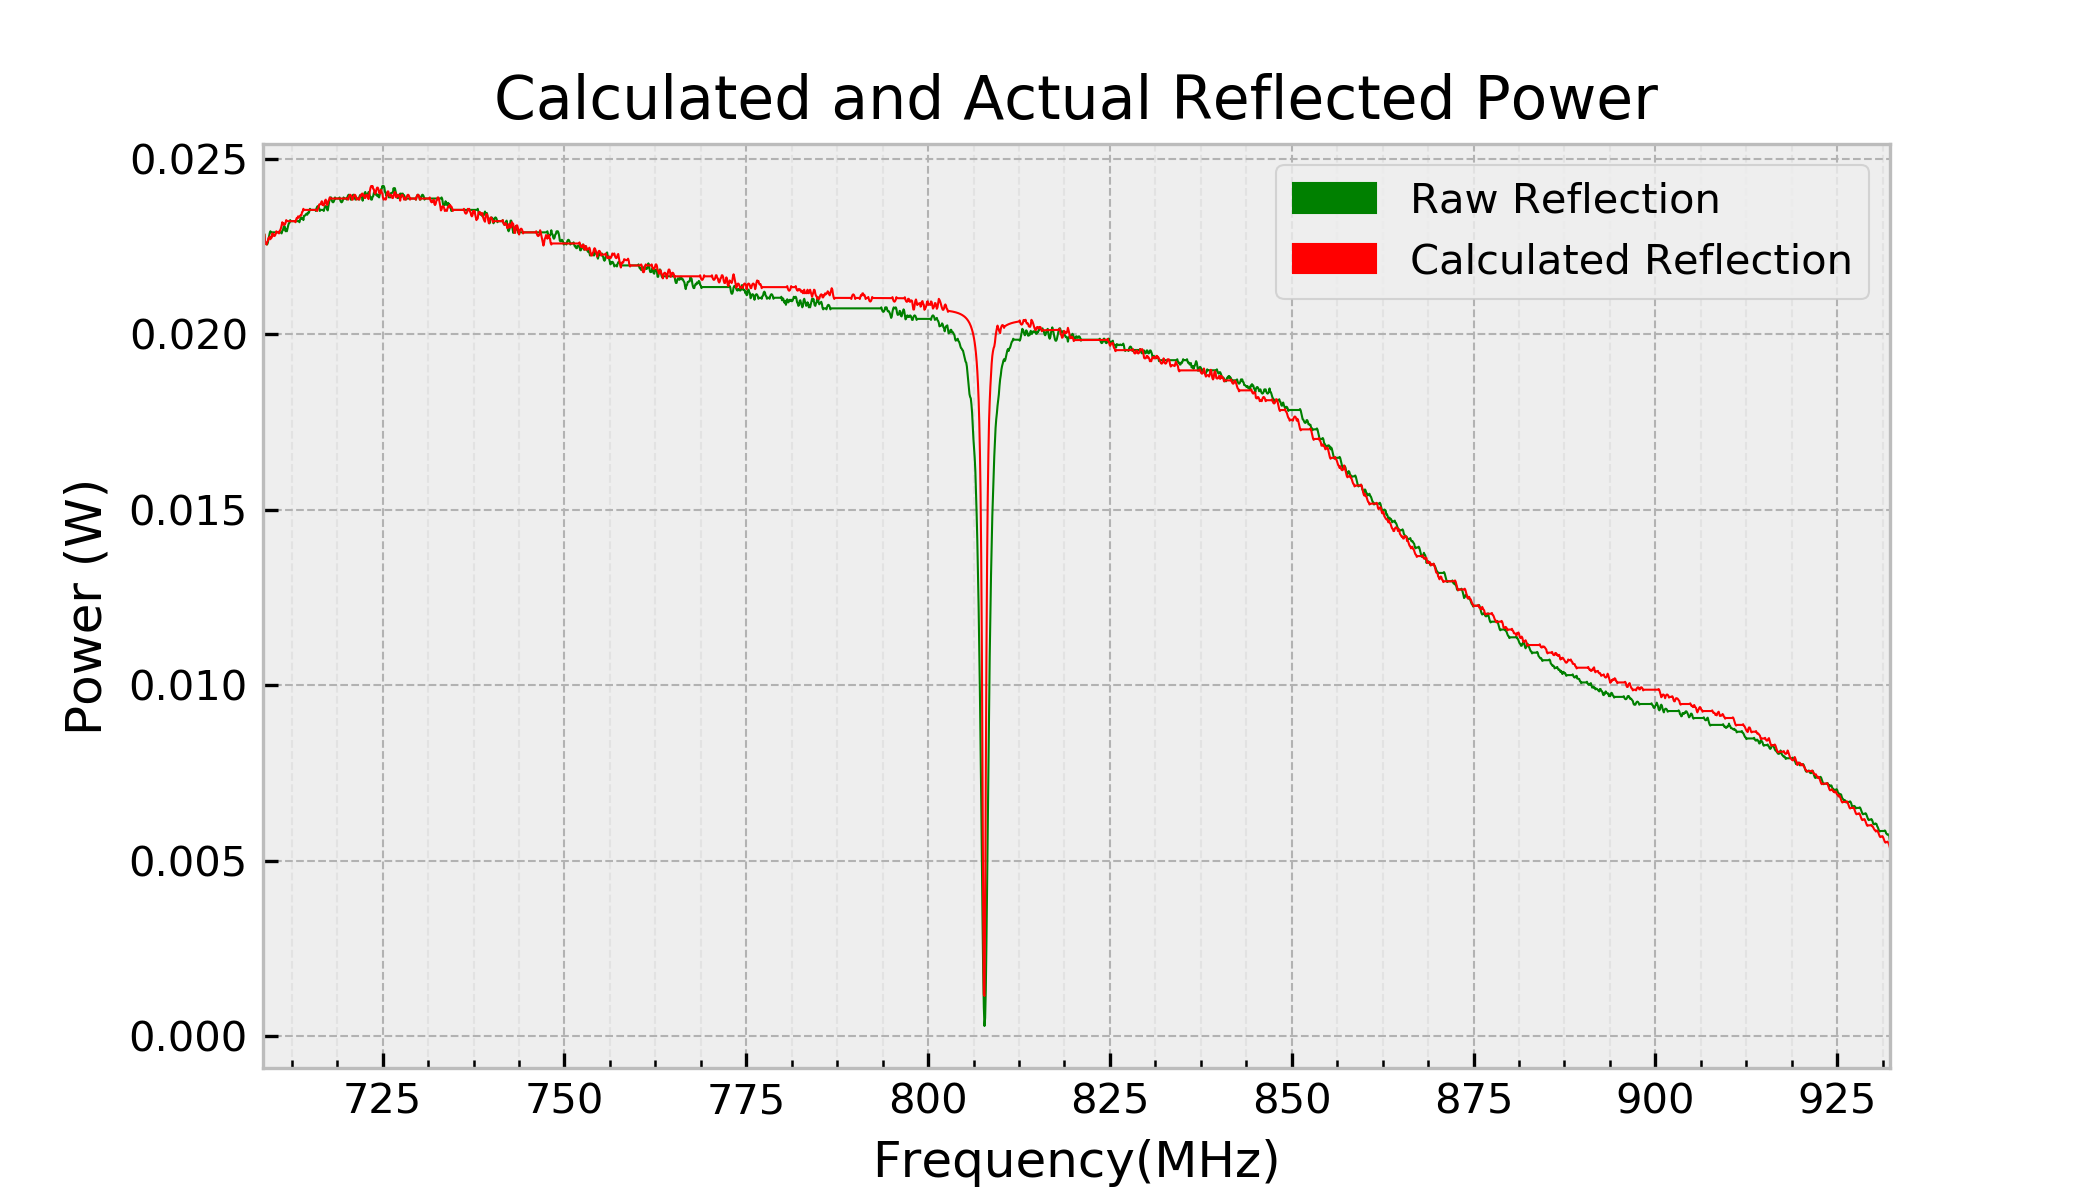
\includegraphics[width=0.95\textwidth]{figures/PartB/reflect_savgol.png}
  \caption{Filtered calculated and raw signals}
 \label{fig:raw_reflect_filt}
\end{subfigure}\hfill
\begin{subfigure}[t]{.475\textwidth}
  \centering
  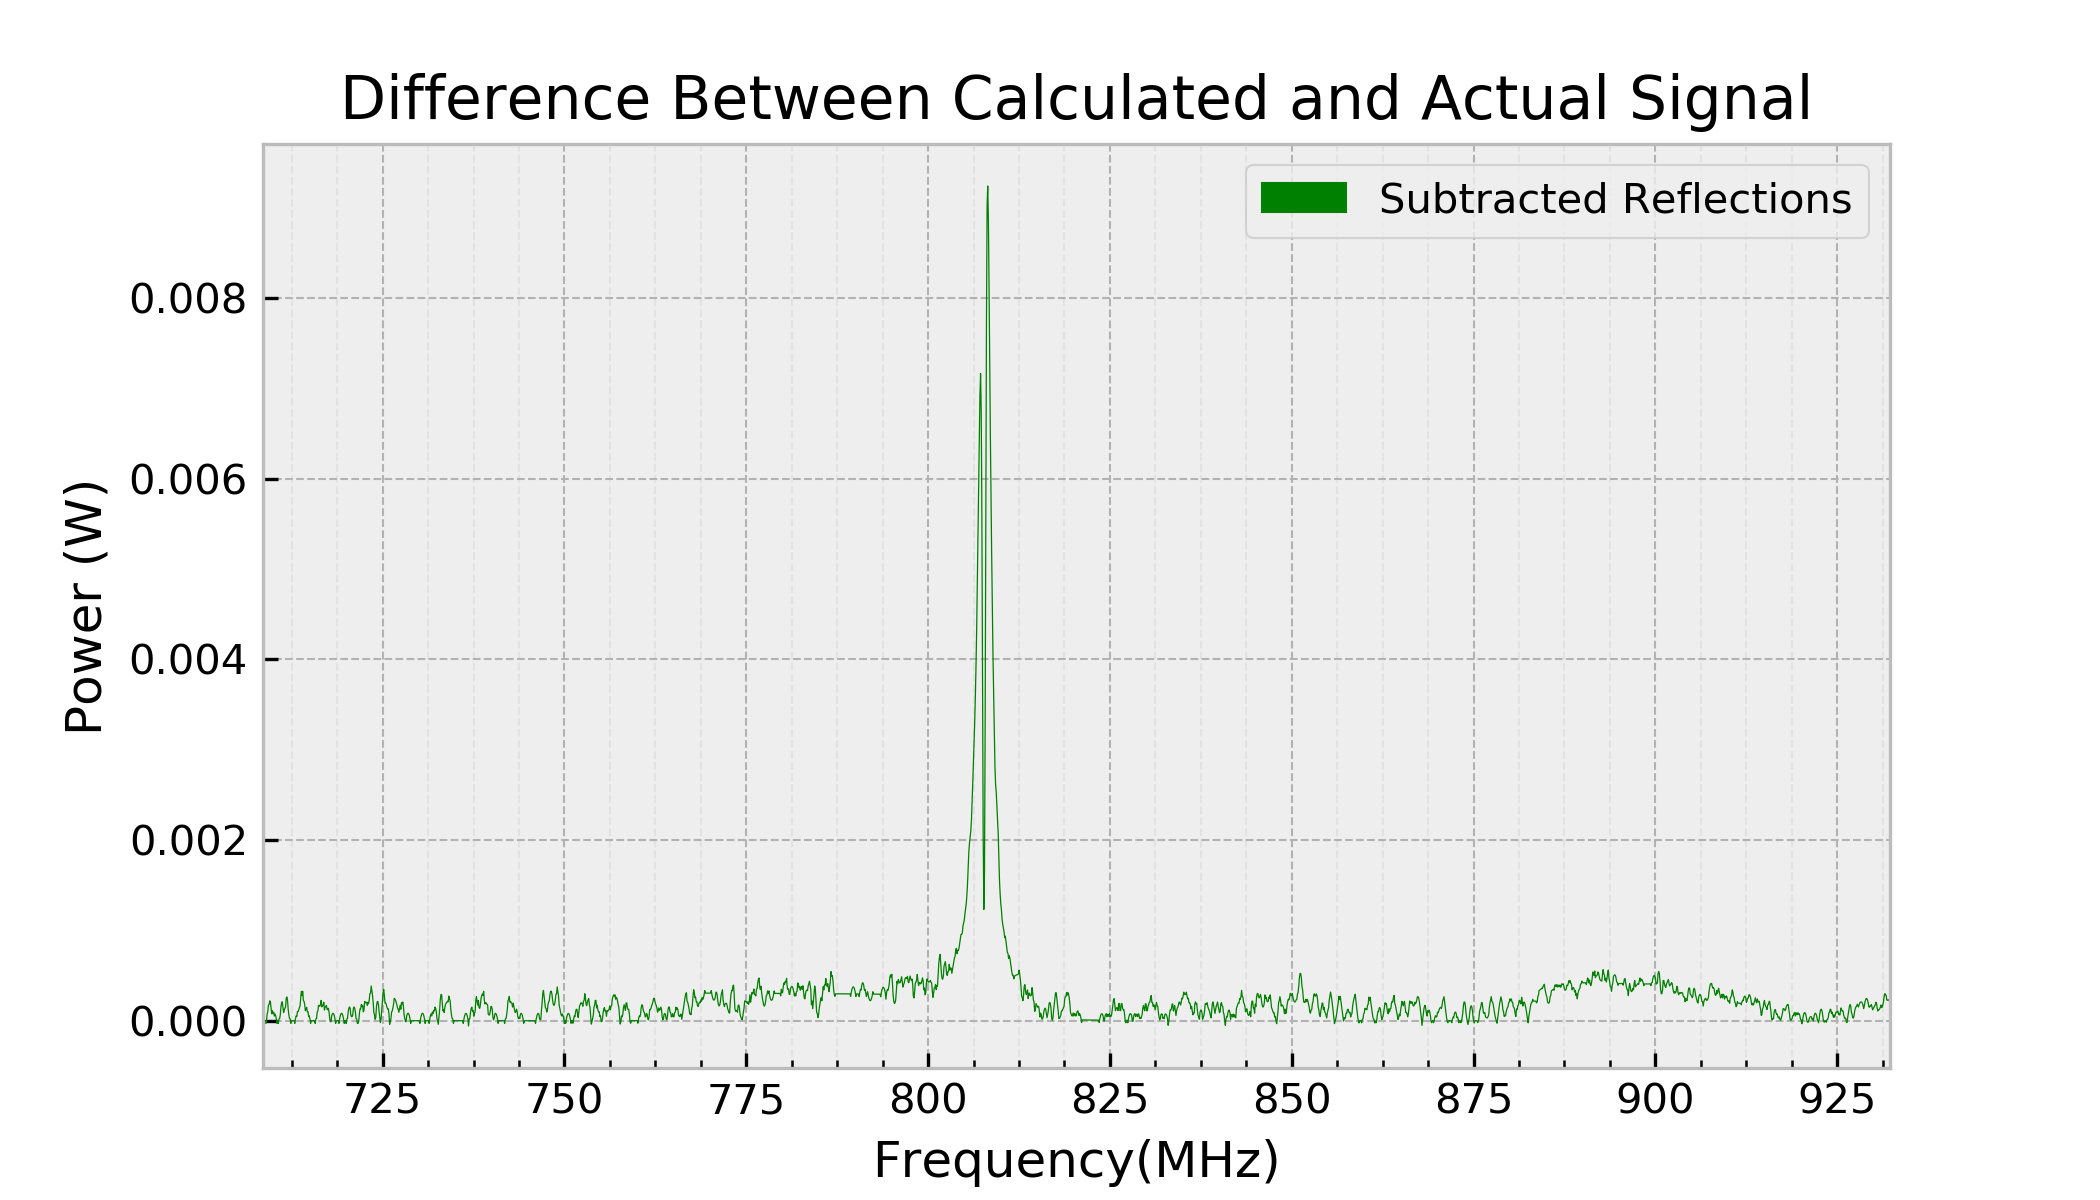
\includegraphics[width=0.95\textwidth]{figures/PartB/reflect_sub.png}
  \caption{Calculated and raw signal subtracted to see difference}
\label{fig:reflect_sub}
\end{subfigure}
\caption{Analysis graphs for the reflected signal}
\label{fig:analysis_reflect}
\end{figure}

As a point of interest we also note that this resonance frequency found of 808 $\pm$ 2 MHz is simply the first resonant frequency. We will note that the reason that the cavity is called a quarter wavelength is that the resonance occurs when the condition $L = \lambda/4$ is satisfied. However we note that from theory we can derive this to be $L/n = \lambda/4$ where n is any positive integer, meaning our first frequency of n=1 $\implies f(n=1)= f_1 = 4/L \implies f(n=2) = 4n/L = 2 \times f_1$. Therefore these higher resonance frequencies will then be n multiples of our found resonant frequency, ex. n=2 $\implies$ 1616 MHz. This also makes sense physically, or in relation to waves in any other medium as any n multiple of a resonant frequency will simply create n-1 nodes in the medium and create resonance at the higher frequency.

\begin{comment}

\begin{figure}[h!]
\centering
\begin{subfigure}[t]{.475\textwidth}
  \centering
  \includegraphics[width=0.95\textwidth]{figures/PartB}
  \caption{comment a}
 \label{fig:a}
\end{subfigure}\hfill
\begin{subfigure}[t]{.475\textwidth}
  \centering
  \includegraphics[width=0.95\textwidth]{figures/PartB}
  \caption{comment b}
\label{fig:b}
\end{subfigure}
\caption{overall comment}
\label{fig:overall}
\end{figure}

\end{comment}